\documentclass[12pt]{article}
\usepackage[left=1cm, right=1cm, top=2cm,bottom=1.5cm]{geometry} 

\usepackage[parfill]{parskip}
\usepackage[utf8]{inputenc}
\usepackage[T2A]{fontenc}
\usepackage[russian]{babel}
\usepackage{enumitem}
\usepackage[normalem]{ulem}
\usepackage{amsfonts, amsmath, amsthm, amssymb, mathtools,xcolor}
\usepackage{blkarray}

\usepackage{tabularx}
\usepackage{hhline}

\usepackage{accents}
\usepackage{fancyhdr}
\pagestyle{fancy}
\renewcommand{\headrulewidth}{1.5pt}
\renewcommand{\footrulewidth}{1pt}

\usepackage{graphicx}
\usepackage[figurename=Рис.]{caption}
\usepackage{subcaption}
\usepackage{float}

%%Наименование папки откуда забирать изображения
\graphicspath{ {./images/} }

%%Изменение формата для ввода доказательства
\renewcommand{\proofname}{$\square$  \nopunct}
\renewcommand\qedsymbol{$\blacksquare$}

%%Изменение отступа на таблицах
\addto\captionsrussian{%
	\renewcommand{\proofname}{$\square$ \nopunct}%
}
%% Римские цифры
\newcommand{\RN}[1]{%
	\textup{\uppercase\expandafter{\romannumeral#1}}%
}

%% Для удобства записи
\newcommand{\MR}{\mathbb{R}}
\newcommand{\MC}{\mathbb{C}}
\newcommand{\MQ}{\mathbb{Q}}
\newcommand{\MN}{\mathbb{N}}
\newcommand{\MZ}{\mathbb{Z}}
\newcommand{\MTB}{\mathbb{T}}
\newcommand{\MTI}{\mathbb{I}}
\newcommand{\MI}{\mathrm{I}}
\newcommand{\MCI}{\mathcal{I}}
\newcommand{\MJ}{\mathrm{J}}
\newcommand{\MH}{\mathrm{H}}
\newcommand{\MT}{\mathrm{T}}
\newcommand{\MU}{\mathcal{U}}
\newcommand{\MV}{\mathcal{V}}
\newcommand{\MB}{\mathcal{B}}
\newcommand{\MF}{\mathcal{F}}
\newcommand{\MW}{\mathcal{W}}
\newcommand{\ML}{\mathcal{L}}
\newcommand{\MP}{\mathcal{P}}
\newcommand{\VN}{\varnothing}
\newcommand{\VE}{\varepsilon}
\newcommand{\dx}{\, dx}
\newcommand{\dy}{\, dy}
\newcommand{\dz}{\, dz}
\newcommand{\dd}{\, d}


\theoremstyle{definition}
\newtheorem{defn}{Опр:}
\newtheorem{rem}{Rm:}
\newtheorem{prop}{Утв.}
\newtheorem{exrc}{Упр.}
\newtheorem{problem}{Задача}
\newtheorem{lemma}{Лемма}
\newtheorem{theorem}{Теорема}
\newtheorem{corollary}{Следствие}

\newenvironment{cusdefn}[1]
{\renewcommand\thedefn{#1}\defn}
{\enddefn}

\DeclareRobustCommand{\divby}{%
	\mathrel{\text{\vbox{\baselineskip.65ex\lineskiplimit0pt\hbox{.}\hbox{.}\hbox{.}}}}%
}
\DeclareRobustCommand{\ndivby}{\mkern-1mu\not\mathrel{\mkern4.5mu\divby}\mkern1mu}


%Короткий минус
\DeclareMathSymbol{\SMN}{\mathbin}{AMSa}{"39}
%Длинная шапка
\newcommand{\overbar}[1]{\mkern 1.5mu\overline{\mkern-1.5mu#1\mkern-1.5mu}\mkern 1.5mu}
%Функция знака
\DeclareMathOperator{\sgn}{sgn}

%Функция ранга
\DeclareMathOperator{\rk}{\text{rk}}
\DeclareMathOperator{\diam}{\text{diam}}


%Обозначение константы
\DeclareMathOperator{\const}{\text{const}}

\DeclareMathOperator{\codim}{\text{codim}}

\DeclareMathOperator*{\dsum}{\displaystyle\sum}
\newcommand{\ddsum}[2]{\displaystyle\sum\limits_{#1}^{#2}}

%Интеграл в большом формате
\DeclareMathOperator{\dint}{\displaystyle\int}
\newcommand{\ddint}[2]{\displaystyle\int\limits_{#1}^{#2}}
\newcommand{\ssum}[1]{\displaystyle \sum\limits_{n=1}^{\infty}{#1}_n}

\newcommand{\smallerrel}[1]{\mathrel{\mathpalette\smallerrelaux{#1}}}
\newcommand{\smallerrelaux}[2]{\raisebox{.1ex}{\scalebox{.75}{$#1#2$}}}

\newcommand{\smallin}{\smallerrel{\in}}
\newcommand{\smallnotin}{\smallerrel{\notin}}

\newcommand*{\medcap}{\mathbin{\scalebox{1.25}{\ensuremath{\cap}}}}%
\newcommand*{\medcup}{\mathbin{\scalebox{1.25}{\ensuremath{\cup}}}}%

\makeatletter
\newcommand{\vast}{\bBigg@{3.5}}
\newcommand{\Vast}{\bBigg@{5}}
\makeatother

%Промежуточное значение для sup\inf, поскольку они имеют разную высоту
\newcommand{\newsup}{\mathop{\smash{\mathrm{sup}}}}
\newcommand{\newinf}{\mathop{\mathrm{inf}\vphantom{\mathrm{sup}}}}

%Скалярное произведение
\newcommand{\inner}[2]{\left\langle #1, #2 \right\rangle }
\newcommand{\linsp}[1]{\left\langle #1 \right\rangle }
\newcommand{\linmer}[2]{\left\langle #1 \vert #2\right\rangle }

%Подпись символов снизу
\newcommand{\ubar}[1]{\underaccent{\bar}{#1}}

%% Шапка для букв сверху
\newcommand{\wte}[1]{\widetilde{#1}}
\newcommand{\wht}[1]{\widehat{#1}}
\newcommand{\ovl}[1]{\overline{#1}}

%%Трансформация Фурье
\newcommand{\fourt}[1]{\mathcal{F}\left(#1\right)}
\newcommand{\ifourt}[1]{\mathcal{F}^{-1}\left(#1\right)}

%%Символ вектора
\newcommand{\vecm}[1]{\overrightarrow{#1\,}}

%%Пространстов матриц
\newcommand{\matsq}[1]{\operatorname{Mat}_{#1}}
\newcommand{\mat}[2]{\operatorname{Mat}_{#1, #2}}

%Оператор для действ и мнимых чисел
\DeclareMathOperator{\IM}{\operatorname{Im}}
\DeclareMathOperator{\RE}{\operatorname{Re}}
\DeclareMathOperator{\li}{\operatorname{li}}
\DeclareMathOperator{\GL}{\operatorname{GL}}
\DeclareMathOperator{\SL}{\operatorname{SL}}
\DeclareMathOperator{\Char}{\operatorname{char}}
\DeclareMathOperator\Arg{Arg}

%Делимость чисел
\newcommand{\modn}[3]{#1 \equiv #2 \; (\bmod \; #3)}


%%Взятие в скобки, модули и норму
\newcommand{\parfit}[1]{\left( #1 \right)}
\newcommand{\modfit}[1]{\left| #1 \right|}
\newcommand{\sqparfit}[1]{\left\{ #1 \right\}}
\newcommand{\normfit}[1]{\left\| #1 \right\|}

%%Функция для обозначения равномерной сходимости по множеству
\newcommand{\uconv}[1]{\overset{#1}{\rightrightarrows}}
\newcommand{\uconvm}[2]{\overset{#1}{\underset{#2}{\rightrightarrows}}}


%%Функция для обозначения нижнего и верхнего интегралов
\def\upint{\mathchoice%
	{\mkern13mu\overline{\vphantom{\intop}\mkern7mu}\mkern-20mu}%
	{\mkern7mu\overline{\vphantom{\intop}\mkern7mu}\mkern-14mu}%
	{\mkern7mu\overline{\vphantom{\intop}\mkern7mu}\mkern-14mu}%
	{\mkern7mu\overline{\vphantom{\intop}\mkern7mu}\mkern-14mu}%
	\int}
\def\lowint{\mkern3mu\underline{\vphantom{\intop}\mkern7mu}\mkern-10mu\int}

%%След матрицы
\DeclareMathOperator*{\tr}{tr}

\makeatletter
\renewcommand*\env@matrix[1][*\c@MaxMatrixCols c]{%
	\hskip -\arraycolsep
	\let\@ifnextchar\new@ifnextchar
	\array{#1}}
\makeatother


%% Переопределение функции хи, чтобы выглядела более приятно
\makeatletter
\@ifdefinable\@latex@chi{\let\@latex@chi\chi}
\renewcommand*\chi{{\@latex@chi\smash[t]{\mathstrut}}} % want only bottom half of \mathstrut
\makeatletter

\setcounter{MaxMatrixCols}{20}

\begin{document}
\lhead{Алгебра-\RN{1}}
\chead{Тимашев Д.А.}
\rhead{Лекция - 18}

\section*{Факториальные кольца}

\begin{defn}
	Целостное кольцо $A$ называется \uwave{факториальным}, если $\forall a \in A, \, a\neq 0, \, a\not\in A^{\times}$ можно разложить в произведение простых множителей единственным образом, с точностью до перестановки множителей и их замены на ассоциированные элементы.
\end{defn}

\textbf{Пример нефакториального целостного кольца}: Рассмотрим кольцо состоящее из всех многочленов над полем $K$, у которых коэффициент при первой степени $x$ равен $0$:
$$
	A = \{f = a_0 + a_2x^2 + a_3x^3 + \dotsc + a_nx^n \mid a_i \in K\}
$$
Легко видеть, что $A \subset K[x]$ - подкольцо. Оно коммутативно, ассоциативно, с единицей и без делителей нуля, но оно не факториально:
$$
	x^6 \in A \Rightarrow x^6 = x^2{\cdot}x^2{\cdot}x^2 = x^3{\cdot}x^3
$$
где $x^2$ - простые элементы в $A$, поскольку их нельзя разложить на многочлены меньшей степени, лежащих в том же самом кольце, то есть не разлагается в произведение двух необратимых множителей. Тоже самое можно сказать и про $x^3$ - простые элементы. $x^2$ и $x^3$ - не ассоциированные элементы и количество множителей в обоих разложениях разное $\Rightarrow$ нарушается единственность разложения на простые множители $\Rightarrow A$ - не факториальное кольцо.

\section*{Неприводимые многочлены}
В прошлый раз мы поняли, что в евклидовом кольце многочленов существует единственное разложение любого многочлена на неприводимые многочлены. Но возникает вопрос, как устроены неприводимые многочлены в $K[x]$? Оказывается, что ответ зависит от поля $K$.

\textbf{Пример}: $f(x) = x^2 + 1$. Этот многочлен неприводим в $\MR[x]$, поскольку он мог бы разложиться на два множителя первой степени, но в этом случае у него были бы корни, но действительных корней у $f(x)$ нет, поскольку $f(x) > 0, \, \forall x \in \MR$. Но $f(x) = (x - i)(x + i)$ в $\MC[x]$. 

Тем не менее есть общие факты, которые справедливы над любым полем.
\begin{prop}(\textbf{Общие факты о неприводимых многочленах для $K[x]$})
	\begin{enumerate}[label=\arabic*)]
		\item Многочлены степени $1$ неприводимы в $K[x]$ для любого $K$;
		\begin{proof}
			Очевидно, поскольку при перемножении степени суммируются, а число $1$ нельзя представить в виде суммы двух меньших натуральных чисел.
		\end{proof}
		\item Неприводимые многочлены степени больше $1$ не имеют корней в $K$;
		\begin{proof}
			Пусть $f(x)$ - неприводимый многочлен степени больше $1$ и у него есть корень $x_0$, тогда по теореме Безу $f(x) = (x - x_0){\cdot}g(x)$. Поскольку $\deg(f) > 1$, тогда $\deg(g) > 0$ и тогда $f$ разложился на два многочлена, каждый из которых необратим $\Rightarrow f(x)$ - приводим.
		\end{proof}
		\item Если многочлены не имеют корней в $K$, то они могут быть приводимыми;
		\begin{proof}
			$f(x) = (x^2 + 1)(x^2 +2)$ - приводим в $\MR[x]$, но не имеет корней в $\MR$;
		\end{proof}
		\item Многочлены наименьшей степени, не имеющие корей в $K$, неприводимы в $K[x]$;
		\begin{proof}
			Пусть $f$ - не имеет корней и имеет самую маленькую степень среди многочленов, которые не имеют корней. Если $f = g{\cdot}h, \, 0 < \deg(g), \deg(h) < \deg(f)$, то $g$ и $h$ тоже не имеют корней $\Rightarrow$ противоречие.
		\end{proof}
	\end{enumerate}	
\end{prop}

\section*{Основная теорема алгебры комплексных чисел (ОТА)}

\begin{theorem}(\textbf{ОТА})
	Любой многочлен $f \in \MC[x]$ степени $>0$ имеет корень в $\MC$.
\end{theorem}
\begin{corollary}
	Неприводимые многочлены в $\MC[x]$ это многочлены $1$-ой степени и только они.
\end{corollary}
\begin{proof}
	Из первого пункта утверждения выше следует, что многочлены первой степени неприводимы, а из второго пункта того же утверждения следует, что неприводимых многочленов степени больше $1$ нет, потому что такой многочлен не имеет корней. В поле комплексных чисел же любой многочлен положительной степени имеет корни $\Rightarrow$ неприводимых многочленов степени больше $1$ не бывает.
\end{proof}
\begin{corollary}
	$\forall f \in \MC[x], \, \deg(f) = n > 0, \, \exists$ разложение в произведение линейных множителей:
	$$
		f(x) = c{\cdot}(x- z_1){\cdot}\dotsc{\cdot}(x - z_n), \, c \neq 0, \, z_1,\dotsc,z_n \in \MC
	$$
	где $c$ - это ненулевой старший коэффициент.
\end{corollary}
\begin{proof}
	Любой многочлен разлагается на неприводимые множители над любым полем, а над полем $\MC$ неприводимые множетели - это только множители первой степени $\Rightarrow$ любой многочлен разлагается на множители первой степени.
\end{proof}
\begin{corollary}
	Число комплексных корней многочлена $f(x) \in \MC[x], \, \deg(f) > 0$, с учетом их кратностей, равно $\deg(f)$.
\end{corollary}
\begin{proof}
	По следствию $2$, корни многочлена $f(x) \in \MC[x], \, \deg(f) =n$ это $z_1,\dotsc, z_n$. Они могут повторяться, причем каждый корень повторяется столько раз, какова его кратность в многочлене $f$ и общее количество равно $n$ с учетом кратностей.
\end{proof}

\begin{defn}
	Поле $K$ называется \uwave{алгебраически замкнутым}, если $\forall f \in K[x]$ степени $>0$ имеет корень в $K$.
\end{defn}
С учетом этого определения, можно более лаконично сформулировать ОТА.
\begin{theorem}(\textbf{ОТА})
	Поле $\MC$ алгебраически замкнуто.
\end{theorem}
\begin{rem}
	Заметим, что следствия верны для любого алгебраически замкнутого поля $K$. Более того, будет верна следующая теорема (без доказательства).
\end{rem}
\begin{theorem}
	Любое поле $K$ можно расширить до алгебраически замкнутого поля $L \supseteq K$.
\end{theorem}
Существует около $10$ доказательств ОТА, одно из первых строгих доказательств было придумано Гауссом, но ни одно из этих доказательств не является чисто алгебраическим, все они в той или иной степени используют аналитические соображения. 
\begin{rem}
	Это так, поскольку $\MC$ само не является чисто алгебраическим объектом, оно строится из $\MR$ с помощью алгебраической конструкции, но $\MR$ строится не чисто алгебраически, оно строится из поля $\MQ$ с помощью аналитической идеи пополнения.
\end{rem}
Доказательство ОТА также не будет чисто алгебраическим, поэтому придется перенести основные простейшие понятия математического анализа с поля $\MR$ на поле $\MC$.

\newpage
\section*{Доказательство ОТА}
\subsection*{Основные понятия математического анализа для $\MC$}
\begin{defn}
	\uwave{$\VE$-окрестностью точки} $z_0$ называется множество чисел: $\MU_\VE(z_0) = \{z \in \MC \mid |z - z_0| < \VE\}$.
\end{defn}
\begin{figure}[H]
	\centering
	\includegraphics[width=0.2\textwidth]{AL1L18_1.png}
	\caption{$\VE$-окрестность точки $z_0$.}
	\label{18_1}
\end{figure}
\begin{defn}
	\uwave{Предел последовательности}: $z_n \to z$ при $n \to \infty$, если: 
	$$
		\forall \VE > 0, \, \exists \, n_0, \, \forall n \geq n_0 \colon z_n \in \MU_\VE(z_0)
	$$
\end{defn}
\begin{figure}[H]
	\centering
	\includegraphics[width=0.2\textwidth]{AL1L18_2.png}
	\caption{Предел последовательности в $\MC$.}
	\label{18_2}
\end{figure}
Предел функции, непрерывность и остальные понятия определяются дословно так же, как для $\MR$, после определения $\VE$-окрестности и предела последовательности.

\subsection*{Основные свойства математического анализа для $\MC$}
Аналогично основным понятиям, основные факты и свойства этих понятий также переносятся с поля $\MR$ на поле $\MC$ вместе с доказательствами без изменений. Отметим лишь некоторые из них.

\begin{lemma}
	Пусть $z_n = x_n + iy_n \to z_0 = x_0 + iy_0$, тогда:
	$$
		z_n \xrightarrow[n\to \infty]{} z_0  \Leftrightarrow x_n \to x_0, \, y_n \to y_0
	$$
\end{lemma}
\begin{proof}\hfill\\
	$(\Rightarrow)$ 
	$$
		|z_n - z_0| = \sqrt{|x_n - x_0|^2 + |y_n - y_0|^2} \geq |x_n - x_0|, |y_n - y_0|  
	$$
	$$
		\Rightarrow |z_n -z_0| \to 0 \Rightarrow |x_n - x_0| \to 0 \wedge |y_n - y_0| \to 0
	$$
	$(\Leftarrow)$ 
	$$
		|x_n -x_0| \to 0 \wedge |y_n - y_0| \to 0 \Rightarrow |z_n - z_0| \to 0
	$$
\end{proof}

\textbf{\uline{Основные свойства}}:
\begin{enumerate}[label=\arabic*)]
	\item \textbf{Неравенство треугольника}: $\forall z_1, z_2 \in \MC, \, |z_1 + z_2| \leq |z_1| + |z_2|$;
	\begin{proof}
		$$
			\forall z_1, z_2 \in \MC, \, |z_1 + z_2|^2 = (z_1 + z_2)(\ovl{z_1} + \ovl{z_2}) = |z_1|^2 + z_1\ovl{z_2} + \ovl{z_1}z_2 + |z_2|^2 =
		$$
		$$	
			= |z_1|^2 + 2\RE(z_1\ovl{z_2})  + |z_2|^2 \leq |z_1|^2 + 2|z_1|{\cdot}|z_2| + |z_2|^2 = (|z_1| + |z_2|)^2 \Rightarrow |z_1 + z_2| \leq |z_1| + |z_2|
		$$
		
	\end{proof}
	\item \textbf{Обратное неравенство треугольника}: $\forall z_1,z_2 \in \MC, \, ||z_1| - |z_2|| \leq |z_1 - z_2|$;
	\begin{proof}
		$$
			\forall z_1,z_2 \in \MC,\, |z_1| = |z_1 - z_2 + z_2| \leq |z_1 - z_2| + |z_2| \Rightarrow |z_1| - |z_2| \leq |z_1 - z_2|
		$$
		$$
			\forall z_1,z_2 \in \MC,\, |z_2| = |z_2 - z_1 + z_1| \leq |z_2 - z_1| + |z_1| \Rightarrow |z_2| - |z_1| \leq |z_2 - z_1| 
		$$
		$$
			|z_2 - z_1| = |z_1 - z_2| \Rightarrow ||z_1| - |z_2|| \leq |z_1 - z_2|	
		$$
	\end{proof}
	\item $z_n \xrightarrow[n\to \infty]{} z \Rightarrow |z_n| \to |z|$;
	\begin{proof}
		$||z_n| - |z|| \leq |z_n - z| \to 0 \Rightarrow |z_n| \to |z|$;
	\end{proof}
	\item $z_n \to z_0, \, w_n \to w_0 \Rightarrow z_n + w_n \to z_0 + w_0$, при $n \to \infty$;
	\item $z_n \to z_0, \, w_n \to w_0 \Rightarrow z_n{\cdot}w_n \to z_0{\cdot}w_0$, при $n \to \infty$;
	\item $f(z) \to f(z_0), \, g(z) \to g(z_0) \Rightarrow f(z) + g(z) \to f(z_0) + g(z_0)$, при $z \to z_0$;
	\item $f(z) \to f(z_0), \, g(z) \to g(z_0) \Rightarrow f(z){\cdot}g(z) \to f(z_0){\cdot}g(z_0)$, при $z \to z_0$;
	\item Если $f$ и $g$ - непрерывны, тогда $f + g$ и $f{\cdot}g$ - тоже будут непрерывными;
\end{enumerate}
\begin{rem}
	Все доказательства, как для $\MR$. 

\end{rem}
\begin{prop}
	Многочлен $f \in \MC[x]$ задает непрерывную функцию $f \colon \MC \to \MC$.
\end{prop}
\begin{proof}
	Следует непосредственно из свойства $5)$: тождественная функция $f(z) = z$ - непрерывна, далее мы берём одночлены и саму эту функцию на себя умножаем $\Rightarrow$ получаем функцию $z^k \Rightarrow$ произведение непрерывных функций - непрерывно. Умножаем на коэффициенты - непрерывность сохраняется, а затем мы получившиеся одночлены складываем $\Rightarrow$ сумма опять будет непрерывной.
\end{proof}

\begin{prop}
	Пусть $K \subset \MC$ - компакт, то есть замкнутое, ограниченное подмножество, тогда любая непрерывная функция $h \colon K \to \MR$ достигает своего минимума в некоторой точке этого компакта.
\end{prop}
\begin{proof}
	Пусть $K \subset \MC$ - компакт. Пусть $M = \inf\limits_{z \in K} h(z)$, она всегда существует у множества вещественых чисел (возможно, что $M = -\infty$). Тогда существует последовательность: $z_n \in K \colon h(z_n) \to M$ при $n \to \infty$.
	\begin{figure}[H]
		\centering
		\includegraphics[width=0.2\textwidth]{AL1L18_3.png}
		\caption{Компакт $K \subset \MC$.}
		\label{18_3}
	\end{figure}
	Вместе с этим, $z_n$ не обязана сходиться. Обозначим её в виде: $z_n = x_n + iy_n$ и рассмотрим в отдельности последовательности действительной части и мнимой. Поскольку $z_n$ - ограниченная, так как $z_n \in K$, то тогда и $x_n$ - ограниченная последовательность $\Rightarrow$ можно выделить сходяющуюся подпоследовательность. Перейдя к ней, без ограничения общности, можно считать, что $x_n \to x_0$ при $n \to \infty$. Аналогично, можно считать, что и $y_n \to y_0$ при $n \to \infty$, тогда: 
	$$
		z_n = x_n + iy_n \xrightarrow[n\to\infty]{} z_0 = x_0 + iy_0 
	$$
	Поскольку $K$ - замкнутое множество, то тогда $\lim\limits_{n \to \infty}z_n = z_0 \in K$. Поскольку $h(z)$ - непрерывна, и поскольку значение этой функции от $z_n$ стремится к $M$, то будет верно:
	$$
		\lim\limits_{n \to \infty}h(z_n) = h(z_0) = M
	$$
	Следовательно, $z_0$ - это точка минимума.
\end{proof}

\subsection*{Доказательство ОТА}
Пусть $f(x) = a_0 + a_1x + \dotsc + a_n x^n \in \MC[x], \, \deg(f) = n > 0$.
\begin{lemma}
	$|f(z)| \to \infty$ при $|z| \to \infty$.
\end{lemma}
\begin{proof}
	Представим $f(z)$ в следующем виде:
	$$
		f(z) = a_0 + a_1z + \dotsc + a_n z^n = z^n{\cdot}\left(\dfrac{a_0}{z^n} + \dfrac{a_1}{z^{n-1}}+ \dotsc + \dfrac{a_{n-1}}{z} + a_n\right) \Rightarrow
	$$
	$$
		\Rightarrow |f(z)| = |z|^n{\cdot}\left| \dfrac{a_0}{z^n} + \dfrac{a_1}{z^{n-1}}+ \dotsc + \dfrac{a_{n-1}}{z} + a_n\right|
	$$
	$$
		\lim\limits_{|z| \to \infty}\left|\dfrac{1}{z}\right| = \lim\limits_{|z| \to \infty}\dfrac{1}{|z|} = 0 \Rightarrow \dfrac{1}{z} \to 0 \Rightarrow \dfrac{a_0}{z^n} + \dfrac{a_1}{z^{n-1}}+ \dotsc + \dfrac{a_{n-1}}{z} \xrightarrow[|z|\to \infty]{} 0
	$$
	Тогда: 
	$$
		\exists \, R > 0 \colon \forall z \in \MC, \, |z| > R \Rightarrow \left| \dfrac{a_0}{z^n} + \dfrac{a_1}{z^{n-1}}+ \dotsc + \dfrac{a_{n-1}}{z}\right| \leq \dfrac{|a_n|}{2} \Rightarrow
	$$
	$$
		\Rightarrow |f(z)| \geq R^n{\cdot}\dfrac{|a_n|}{2} \xrightarrow[R \to \infty]{} \infty \Rightarrow \forall C> 0, \, \exists\, R > 0, \, \forall |z|  \geq R \colon |f(z)| > C \Rightarrow |f(z)| \xrightarrow[|z| \to \infty]{} \infty
	$$
\end{proof}
\newpage
\begin{lemma}(\textbf{Даламбера})
	Если $z_0\in \MC, \, ,f(z_0) \neq 0$, тогда $\forall \VE > 0, \, \exists \, z \in \MU_{\VE}(z_0)\colon |f(z)| < |f(z_0)|$.
\end{lemma}
\begin{rem}
	Лемма Даламбера неформально говорит, что ненулевое значение многочлена всегда можно уменьшить по модулю.
\end{rem}
\begin{proof}
	Разложим многочлен $f(x)$ по степеням $x - z_0$, пропустив те члены, которые будут равны нулю:
	$$
		f(x) = c_0 + c_k{\cdot}(x - z_0)^k + (x - z_0)^{k+1}{\cdot}g(x), \quad c_0, c_k \neq 0
	$$
	Ненулевой коэффициент $c_k$ найдется, иначе многочлен $f$ был бы константой, а у нас $\deg(f) > 0$. Также, заметим, что $c_0 \neq 0$ потому, что $f(z_0) = c_0 \neq 0$. После $c_k$ также могут идти ненулевые коэффициенты, мы их объединили и вынесли общий множитель $(x - z_0)^{k+1}$, всё остальное объединили в $g(x)$. Подберём число $z \in \MU_{\VE}(z_0)$ так, чтобы: 
	$$
		\Arg(c_k(z- z_0)^k) = \Arg(c_0) + \pi
	$$ 
	Два вектора имеют противоположное направление $\Rightarrow$ комплексные числа имеют аргумент отличающийся на $\pi$. При этом, мы хотим, чтобы:
	$$
		|c_k(z-z_0)^k| < |c_0|
	$$
	Пусть $\varphi = \Arg(c_0)$, $\psi = \Arg(c_k)$ и $z - z_0 = r{\cdot}e^{i\alpha}$, где $r$ - фиксированно.
	\begin{figure}[H]
		\centering
		\includegraphics[width=0.35\textwidth]{AL1L18_4.eps}
		\caption{Доказательство леммы Даламбера.}
		\label{18_4}
	\end{figure}
	Перепишем условия выше:
	$$
		\begin{cases}
			\Arg(c_k(z- z_0)^k) = \Arg(c_0) + \pi\\
			|c_k(z-z_0)^k| < |c_0|
		\end{cases}\Leftrightarrow
		\begin{cases}
			\psi + k{\cdot}\alpha = \varphi + \pi\\
			|c_k|{\cdot}r^k < |c_0|
		\end{cases} \Leftrightarrow
		\begin{cases}
			\alpha = \dfrac{\varphi + \pi - \psi }{k}\\[8pt]
			r < \sqrt[k]{\tfrac{|c_0|}{|c_k|}}
		\end{cases}
	$$
	Подобрав $z$, удовлетворяющее условиям выше, мы получим следующее:
	$$
		|c_0 + c_k(z - z_0)^k| < |f(z_0)|
	$$
	При достаточно малом $r$, третий член разложения будет меньше любого заданного нами числа:
	$$
		|(z - z_0){\cdot}g(z)| = r{\cdot}|g(z)| < |c_k| \Rightarrow |(z - z_0)^{k+1}{\cdot}g(z)| < |c_k{\cdot}(z - z_0)^k|
	$$
	поскольку $g(z)$ - многочлен $\Rightarrow$ непрерывная функция, а непрерывная функция в окрестности точки $z_0$ будет ограничена, в том числе и по модулю. Таким образом, точка $f(z)$ лежит внутри окружности радиуса $|c_k(z - z_0)^k|$ с центром в точке $f(z_0) + c_k(z - z_0)^k$. Тогда точка $f(z)$ попадет внутри окружности с центром в нуле, радиуса $|f(z_0)|$, в частности это означает: $|f(z)| < |f(z_0)|$. Алгебраически:
	$$
		|f(z)| \leq |c_0 + c_k(z -z_0)^k| + |(z - z_0)^{k+1}{\cdot}g(z)| = 
	$$
	$$
		=|c_0| - |c_k(z - z_0)^k| + |(z - z_0)^{k+1}{\cdot}g(z)| < |c_0| = |f(z_0)|
	$$
\end{proof}

\textbf{\uline{Доказательство ОТА}}:
\begin{proof}\hfill
	\begin{enumerate}[label=\arabic*)]
		\item Покажем, что $|f(z)|$ достигает минимума на $\MC$ в некотрой точке $z = z_0$. По лемме $2$, $|f(z)| \to \infty$, когда $|z| \to \infty$, тогда:
		$$
			\exists \, R > 0 \colon \forall z \in \MC, \, |z| > R \Rightarrow |f(z)|  > |a_0|
		$$
		У нас получается замкнутый круг радиуса $R$ на комплексной плоскости, за пределами которого значение многочлена по модулю достаточно большое. Обозначим его так: 
		$$
			K = \{z \in \MC \mid |z| \leq R\}
		$$
		Что происходит внутри? На компакте $K$ $|f(z)|$ достигает минимума в некоторой точке $z = z_0 \in K$.
		\begin{figure}[H]
			\centering
			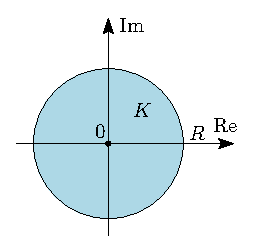
\includegraphics[width=0.25\textwidth]{AL1L18_5.eps}
			\caption{Компакт $K$.}
			\label{18_5}
		\end{figure}
		На самом деле это будет минимум и на всей плоскости. В самом деле:
		$$
			\forall z \in K, \, |f(z)| \geq |f(z_0)| \Rightarrow |f(0)| = |a_0| \geq |f(z_0)|
		$$
		$$
			\forall z \not\in K,\, |f(z)| > |a_0| \geq |f(z_0)|
		$$
		Следовательно, $z_0$ - это точка минимума на $\MC$;
		\item Убедимся, что $f(z_0) = 0$. Если $f(z_0) \neq 0$, то по лемме Даламбера: $\exists \, z \in \MC \colon |f(z)| < |f(z_0)|$, но это противоречие, поскольку $z_0$ - это точка минимума $\Rightarrow f(z_0) = 0$;
	\end{enumerate}
\end{proof}
\newpage
\section*{Многочлены над полем $\MR$}
Как устроены неприводимые многочлены, разложение на неприводимые множители в $\MR[x]$?
\begin{lemma}
	Пусть $f \in \MR[x]$, тогда $z_0 \in \MC$ является корнем $f$ кратности $k \Leftrightarrow \ovl{z}_0$ - корень $f$ кратности $k$.
\end{lemma}
\begin{proof}
	$$
		f(x) = a_0 + a_1x + \dotsc + a_n x^n, \, \forall i =\ovl{0,n}, \, a_i \in \MR
	$$
	$$
		\forall z \in \MC, \, f(z) = a_0 + a_1z+ a_2 z^2 + \dotsc + a_n z^n \Rightarrow \ovl{f(z)} = \ovl{a}_0 + \ovl{a_1z} + \ovl{a_2z^2} + \dotsc+ \ovl{a_nz^n} = 
	$$
	$$
		= a_0 + a_1\ovl{z} + a_2\ovl{z}^2	+ \dotsc + a_n\ovl{z}^n = f(\ovl{z}) \Rightarrow f(z_0) = 0 \Leftrightarrow f(\ovl{z}_0) = 0
	$$
	Аналогично, мы можем получить, что: 
	$$
		\forall k \in \MN, \, f^{(k)}(z_0) = 0 \Leftrightarrow f^{(k)}(\ovl{z}_0) = 0
	$$
	Таким образом, $z_0$ - корень $f$ кратности $k \Leftrightarrow f(z_0) = f'(z_0) = \dotsc = f^{(k-1)}(z_0) = 0 \neq f^{(k)}(z_0)$, но поскольку это эквивалентно обращению в нуль для каждой из производной в $\ovl{z}_0$, то:
	$$
		f(z_0) = f'(z_0) = \dotsc = f^{(k-1)}(z_0) = 0 \neq f^{(k)}(z_0) \Leftrightarrow f(\ovl{z}_0) = f'(\ovl{z}_0) = \dotsc = f^{(k-1)}(\ovl{z}_0) = 0 \neq f^{(k)}(\ovl{z}_0)
	$$
	А это означает, что $\ovl{z}_0$ - тоже корень $f$ кратности $k$.
\end{proof}

\begin{theorem}
	Неприводимые многочлены в $\MR[x]$ - это многочлены первой степени и многочлены второй степени с отрицательным дискриминантом. Любой многочлен в $\MR[x]$ степени $> 0$ разлагается в произведение линейных множителей (отвечающих его действительным корням) и квадратичных множителей с отрицательным дискриминантом (отвечающих парам сопряженных мнимых корней).
\end{theorem}
\begin{proof}
	Разложим $f \in \MR[x]$ на линейные множители (то есть, множители первой степени) над $\MC$:
	$$
		f(x) = c(x - x_1){\cdot}\dotsc{\cdot}(x - x_r){\cdot}(x - z_1){\cdot}(x - \ovl{z}_1){\cdot}\dotsc{\cdot}(x - z_k){\cdot}(x - \ovl{z}_k){\cdot}\dotsc{\cdot}(x - z_s){\cdot}(x - \ovl{z}_s)
	$$
	$$
		x_1,\dotsc, x_r \in \MR, \, z_1, \dotsc, z_s \in \MC \setminus \MR
	$$
	$$
		\forall k = \ovl{1,s}, \, (x - z_k){\cdot}(x - \ovl{z}_k)= x^2 - (z_k + \ovl{z}_k)x + z_k\ovl{z}_k = x^2 - 2\RE(z_k) + |z_k|^2 \in \MR[x]
	$$
	Мы получили квадратный трехчлен с действительными коэффициентами. Посчитаем его дискриминант:
	$$
		\dfrac{D}{4} = \RE(z_k)^2 - |z_k|^2 = - \IM(z_k)^2 < 0
	$$
	Линейные и квадратичный множители дальше над $\MR$ не разлагаются $\Rightarrow$ они неприводимые.
\end{proof}

\begin{corollary}
	$f \in \MR[x], \, \deg(f)$ - нечетная, тогда $f(x)$ имеет корень в $\MR$.
\end{corollary}
\begin{proof}
	В разложении на неприводимые множители все множители не могут быть квадратичными. Тогда есть линейный множитель $\Leftrightarrow$ есть вещественный корень. Ещё это можно показать так:
	$$
		f(x) = x^{2n + 1} + a_{2n}x^{2n} + \dotsc + a_1x + a_0 \Rightarrow f(x) \xrightarrow[x \to +\infty]{} + \infty, \, f(x) \xrightarrow[x \to -\infty]{}  -\infty
	$$
	По теореме о промежуточном значении непрерывной функции, многочлен примет значение $0$, а это и значит, что есть вещественный корень.
\end{proof}

\end{document}